%----------------------------------------------------------------------------------------
%
% LaTeX-template for degree projects at LNU, Department of Computer Science
% Last updated by Johan Hagelbäck, Mar 2017
% Linnaeus University
%
% License: Creative Commons BY
%
%----------------------------------------------------------------------------------------

%----------------------------------------------------------------------------------------
%	Settings and configuration
%----------------------------------------------------------------------------------------

\documentclass[a4paper,12pt]{article}

\usepackage[T1]{fontenc}
\usepackage{times}
\usepackage[english]{babel}
\usepackage[utf8]{inputenc}
\usepackage{dtklogos}
\usepackage{wallpaper}
\usepackage[absolute]{textpos}
\usepackage[top=2cm, bottom=2.5cm, left=3cm, right=3cm]{geometry}
\usepackage{appendix}
\usepackage[nottoc]{tocbibind}
\usepackage[colorlinks=true,
            linkcolor=black,
            urlcolor=blue,
            citecolor=black]{hyperref}

\setcounter{secnumdepth}{3}
\setcounter{tocdepth}{3}

\usepackage{sectsty}
\sectionfont{\fontsize{14}{15}\selectfont}
\subsectionfont{\fontsize{12}{15}\selectfont}
\subsubsectionfont{\fontsize{12}{15}\selectfont}

\usepackage{csquotes} % Used to handle citations

\renewcommand{\thetable}{\arabic{section}.\arabic{table}}  
\renewcommand{\thefigure}{\arabic{section}.\arabic{figure}} 

%----------------------------------------------------------------------------------------
%	
%----------------------------------------------------------------------------------------
\newsavebox{\mybox}
\newlength{\mydepth}
\newlength{\myheight}

\newenvironment{sidebar}%
{\begin{lrbox}{\mybox}\begin{minipage}{\textwidth}}%
{\end{minipage}\end{lrbox}%
 \settodepth{\mydepth}{\usebox{\mybox}}%
 \settoheight{\myheight}{\usebox{\mybox}}%
 \addtolength{\myheight}{\mydepth}%
 \noindent\makebox[0pt]{\hspace{-20pt}\rule[-\mydepth]{1pt}{\myheight}}%
 \usebox{\mybox}}

%----------------------------------------------------------------------------------------
%	Title section
%----------------------------------------------------------------------------------------
\newcommand\BackgroundPic{
    \put(-2,-3){
    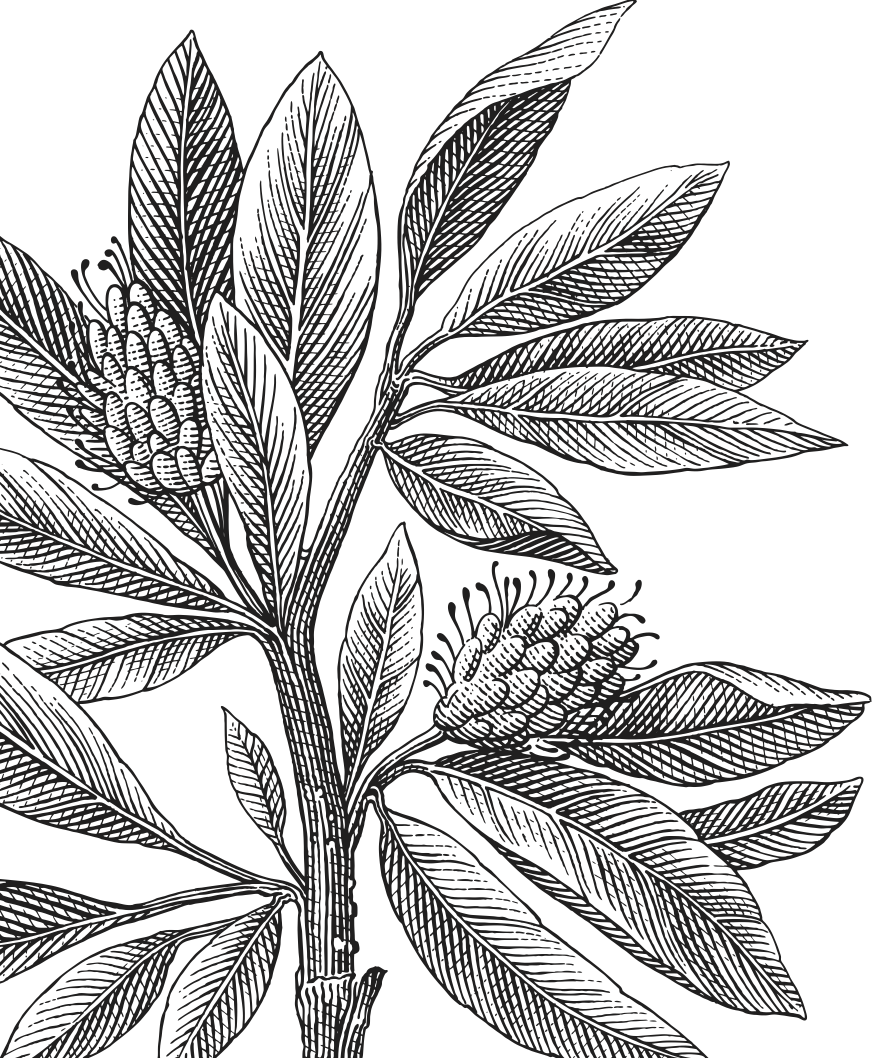
\includegraphics[keepaspectratio,scale=0.3]{img/lnu_etch.png} % Background picture
    }
}
\newcommand\BackgroundPicLogo{
    \put(30,740){
    
\includegraphics[keepaspectratio,scale=0.10]{img/logo.png} % Logo in upper left corner
    }
}

\title{	
\vspace{-8cm}
\begin{sidebar}
    \vspace{10cm}
    \normalfont \normalsize
    \Huge Bachelor Degree Project \\
    \vspace{-1.3cm}
\end{sidebar}
\vspace{3cm}
\begin{flushleft}
    \huge Evaluation of improvement measures of DNS Privacy\\ 
    \it \LARGE - Protection towards Web filters 
\end{flushleft}
\null
\vfill
\begin{textblock}{6}(10,13)
\begin{flushright}
\begin{minipage}{\textwidth}
\begin{flushleft} \large
\emph{Author:} Songho Lee\\ % Author
\emph{Supervisor:} Ola Flygt\\ % Supervisor
%\emph{Examiner:} Dr.~Mark \textsc{Brown}\\ % Examiner (course manager)
\emph{Semester:} VT 2019\\ % 
\emph{Subject:} Computer Science\\ % Subject area
\end{flushleft}
\end{minipage}
\end{flushright}
\end{textblock}
}

\date{} 

\begin{document}
\pagenumbering{gobble}
\newgeometry{left=5cm}
\AddToShipoutPicture*{\BackgroundPic}
\AddToShipoutPicture*{\BackgroundPicLogo}
\maketitle
\restoregeometry
\clearpage
%----------------------------------------------------------------------------------------
%	Abstract
%----------------------------------------------------------------------------------------
\selectlanguage{english}
\begin{abstract}
\noindent The report shall begin with a summary, called abstract. The abstract shall not be longer than a paragraph, and is not divided into more than one piece. It shall contain:

\begin {itemize}
\item A short background description to the area of your project
\item A description of the problem you investigate
\item A motivation why this problem is interesting to investigate
\item What you have done to answer the problem
\item A short summary of your results
\end {itemize}

From reading the abstract the reader should clearly understand what the report is all about. The purpose of the abstract is to make the reader interested in continue reading the report, if it covers something that the reader wants to know more about.
\newline
\newline
\textbf{Keywords: DNS, DNS-over-https, DNS-over-TLS, Privacy}
\end{abstract}

\newpage
%----------------------------------------------------------------------------------------
%	Preface
%----------------------------------------------------------------------------------------

\textbf {\large{Preface}}\\

\noindent You can have a preface in the report if you want, but it is not necessary. In this you can write more personal reflections on your degree project. In the preface you can also take the opportunity to thank the people who have been particularly helpful during the report writing, for example if you had any contact with a company that helped with the project, people that guided or helped you during the project, or your family and friends that supported you during the project. The preface shall not be longer than half a page.

%----------------------------------------------------------------------------------------
\newpage
\pagenumbering{gobble}
\tableofcontents % Table of contents
\newpage
\pagenumbering{arabic}

%----------------------------------------------------------------------------------------
%
%	Here follows the actual text contents of the report.
%
%----------------------------------------------------------------------------------------

\section{Introduction}
In this chapter you shall give an introduction to your degree project. It shall start with a broad overview of what your project is all about. Similar to the abstract, the introduction shall make the reader interested in continue reading your report. Don't be too detailed here; there are plenty of opportunities to add details in later chapters.

\subsection{Background}
``Pervasive Monitoring is a widespread attack on privacy\cite{rfc7258}.'' Information collected in such action could lead to a breach of users’ privacy, by re-identifying users based on traffic\cite{herrmann2010analyzing}, or could become aids for launching an active form of attacks, such as masquerade and denial of service.

A commonly found practical example of the large scale monitoring is a web filter\cite{murdoch2008tools}. Wazen et. al categorise legacy web-filtering techniques as following: (a) Port-based, (b) DNS, (c) IP Address, (d) Certificate, (e) Payload-based (f) HTTP proxy filtering techniques\cite{shbair2015efficiently}.

Among the various types of filtering techniques mentioned above, methods (a) and (c) are considered less efficient due to changes in the Internet ecosystem in recent decennial;
Internet firms such as Google, Facebook and Amazon show strong presence\cite{haucap2014google}, and the phenomenon may have reduced the diversity of traffic endpoint's IP addresses.
Moreover, it has become more common to have web services deployed in cloud environments\cite{clouds2018stat}, and IaaS providers extensively use ``Virtual Host\cite{virtual24host}'', which means various Web servers correspond to the same IP address.
It also eliminates the need for utilising different ports to co-host services. Thus, port usages are normalised.

Also, another notable change of the Internet is that adoption of HTTPS on the web has increased significantly\cite{felt2017measuring}.
The change has increased costs of performing technique (e) and brought challenges in payload-based traffic classification \cite{xue2013traffic}.
Also, it has made (f) less applicable, as a proxy does not directly processes encrypted traffics\cite{shbair2015efficiently}.
Furthermore, the combination of wide deployment of HTTPS and Virtual Hosting has made technique (e) inefficient, because ``many companies share the same certificate across different services and domain names\cite{shbair2015efficiently}''.

However, the trend change of Internet has not brought additional challenges to Domain Name System (DNS) filtering. Currently, almost all DNS traffic is sent in clear text \cite{rfc7626} over the UDP protocol \cite{tcp2014analysis}, and it makes DNS queries vulnerable to being hijacked and filter users' traffic.

\subsection{Related work}
The project accredits pioneer researches which has provided thorough evaluation of options to improve DNS Privacy. 
Patrick Werneck evaluated approaches to improve privacy of DNS and stated limitations of identified approaches\cite{werneck2014dns} in 2014.
J.H.C. van Heugten evaluated exisiting solutions to ehnance DNS Privacy in 2018 in his study \cite{van2018privacy}. As standariseation of DNS-over-HTTPS is recently finalised\cite{rfc8484}, study from van Heugten reflects more recent changes.

\subsection{Problem formulation}
S. Bortzmeyer has claimed in RFC 7626, the informational note on DNS privacy\cite{rfc7626}, that particular fields in DNS packet\cite{rfc1035} such as Query name  (QNAME) and Source IP address reveal ``communication relationships''. By enumerating the DNS query process, we identify risks of such information leakage in following places: (1) tapping on the wire, ``between the stub resolvers and the recursive resolvers'', and (2) information leaks in the servers, such as in Recursive resolvers, Authoritative name servers and Rogue recursive resolvers. This project aims to answer the following research questions.
\\\\
\begin{tabular} {|p{1.2cm}|p{11.6cm}|} \hline
  \textbf{RQ1} & What methods exist to enhance DNS Privacy? \\ \hline
  \textbf{RQ2} & How does DNS Privacy improvement benefit users from being blocked by web filters?\\ \hline
  \textbf{RQ3} & What would be possible disadvantages or overheads with DNS Privacy enrichment? \\ \hline
  \end{tabular}

\subsection{Motivation}
Most of the internet activities begin with DNS query, hence DNS is vital. Notwithstanding the importance of DNS, designers of the current DNS protocol have not taken consideration of ``confidentiality of protocol metadata''. Therefore DNS queries reveal communication flows, and this property of DNS protocol is used in different contexts by different actors. Examples of usages are traffic monitoring for network management or limiting the influence of malicious websites by DNS Footprinting of malware\cite{stoner2010dns}, or detecting malware infections\cite{lemos2013got}.

Other exemplary usages of this property of DNS are nation-state surveillance, privacy-unfriendly activities of commercial sectors\cite{weaver2011redirecting}, and illegal actions by criminals. Surveillance affects individuals to possess stress and anxiety\cite{oulasvirta2012long}, and behavioural changes like self-censorship \cite{rfc6973}. RFC 6973 connotes that Privacy harms involve ``harms to financial standing, reputation, solitude, autonomy, and safety\cite{rfc6973}''.

S. Farrell et al. state in RFC 7258 that allowing monitoring by benevolent actors and defending privacy against nefarious actors do not hold hand in hand, as the actions required to achieve both, regardless of the motivations, are indistinguishable\cite{rfc7258}.
Disadvantages incurred by lack of DNS privacy significantly overweight advantages, and therefore DNS privacy should be mitigated in any feasible practices.

\subsection{Objectives}
Present a list of the objectives to do in your project. An objective shall be understandable, not too small or too large, and possible to define when it is completed or not. You have already defined objectives in your project plan. Copy and paste them here. You can read more about objectives \href{https://coursepress.lnu.se/subject/thesis-projects/objectives/}{here}.\\

\begin{tabular} {|p{1.2cm}|p{11.6cm}|} \hline
    \textbf{O1} & Explore the state of arts in mitigative methods to enhance DNS Privacy \\ \hline
    \textbf{O2} & Verify application of DNS privacy-enhancing methods complicates DNS eavesdropping\\ \hline
    \textbf{O3} & Identify areas which the selected methods could not address. \\ \hline
    \textbf{O4} & Estimate factors that may lead to a load increase on recursive DNS resolvers by improving DNS Privacy.\\ \hline
\end{tabular}\\

\subsection{Scope/Limitation}
The project has a focus on improving privacy part, from the security perspectives. In other words, reflected to a CIA triad, enhancing Integrity and availability perspective is not priortised in the current project. Issues and challenges of DNS security as whole may be found in other studies, such as one conducted by Ning Hu et. al.\cite{ning2017dnssecurity}. 

You cannot solve everything. Here you describe what you do, and what you don't do, in your project. Limitations can for example be that you only compare some frameworks of all frameworks available on the market, that you only suggest an architecture for a specific software product and not a general architecture, or that you only include university students in a study and not a broader population sample.

\subsection{Target group}
Criticism
1. Only shift of the reliability
The project aims to provide insight on DNS Privacy for Internet users and recursive resolver providers for improving users' privacy.
Here you outline which target group that might be interested in your work. If you, for example, do a project about software architectures, a target group can be professional developers and architects that work with similar software systems as the system you investigated.

\subsection{Outline}
Here you outline the rest of the report. It shall contain which chapters that will follow, and what each of them is about.

\newpage
\
\section{Method}
\label{Method}
The project is anticipated to be done in following scientific methods.
\begin{itemize}
\item Literature Review
\item Controlled Experiment
\end{itemize}
There is a need for performing a systematic literature review to accomplish \textbf{O1}. As RFC 7626\cite{rfc7626} provides a clear insight of DNS privacy issues and as around four years have passed since its publication, it is anticipated that fellow researchers have tried to solve or list risks identified in the article. Therefore, search criterium is to list articles that cite RFC 7626 from a database Google Scholar. Once articles are identified, these will fall into categories and selected by exclusion criteria.
%If the results based on the criteria is insufficient, inclusive criteria will be applied using search term such as DNS Privacy and DNS Security will be used. Exclusive criteria must be applied as well to limit the contents of the articles to be relevant to the defined problem. Therefore, any solving other security aspects of DNS, such as availability or integrity will be excluded.
The expected outcome of \textbf{O1} is a set of measurements to enhance DNS privacy.

\textbf{O2} is accomplished by selecting securing methods that are near or already in practice and reproduce these in a controlled environment. Due to this reason, it may exclude some of the areas from \textbf{O1}. Verification, as defined in \textbf{O2}, is done by Examining DNS query and response packets between stub resolver and recursive resolver, after having applied privacy enhancive methods under the controlled environment. If the time allows, Deep Packet Inspection(DPI) middleware could optionally be deployed in the environment and see results of analysis of the secured DNS query process.

\textbf{O3} is achieved by studying surveys from \textbf{O1} and empirical results from \textbf{O2}. \textbf{O4} is evaluated based on outcome of \textbf{O1} and \textbf{O2}.

\subsection{Reliability and Validity}
Here you discuss the reliability and validity of your project. To answer your problem you use a method, collect (and possibly analyze) data, and draw conclusions from the data. 

Reliability means if others will get the same result as you if they replicate your work. Reliability problems can, for example, occur if you use the wrong method for data collection.

It is important that you only draw conclusions that are valid, i.e. that is supported by the way you have done your work and the data you have collected. 

You can read about reliability \href{https://coursepress.lnu.se/subject/thesis-projects/reliability/}{here} and about validity \href{https://coursepress.lnu.se/subject/thesis-projects/validity/}{here}. Discuss if you have any reliability issues or validity threats in your project here.

\subsection{Ethical considerations}
You are required to discuss any ethical considerations (if any) in your project. If you do an experiment you will most likely not have any ethical considerations, but in a survey ethical considerations can for example be how you make sure that the privacy of the people participating in the study is not violated (by for example removing names from the gathered data). 

\newpage

\section{Implementation}
It is common that you will develop something in your project. It can be a mobile app, a stand-alone application, a website, a game, etc. In this chapter you describe the software you have implemented. 

In some projects you don't develop anything, for example if you do a systematic literature review. In this case you remove this chapter.

\newpage

\section{Results}
In this chapter you show and describe your results. You shall only show the raw results without any analysis, and you shall not put any conclusions or opinions in the description of the results. Try to be as objective as possible. An example of results from an experiment comparing five sorting algorithms is shown in Table \ref{results} below.\\

\begin{center}
\begin{table}[ht]
\begin{center}
\begin{tabular}{ccccccc}
\hline
Run & Bubble & Quick & Selection & Insertion & Merge \\
\hline
1 & 17384 & 24 & 3258 & 3 & 30 \\
2 & 17559 & 21 & 3386 & 3 & 27 \\
3 & 17795 & 19 & 3344 & 4 & 28 \\
4 & 17484 & 20 & 3417 & 3 & 28 \\
5 & 17642 & 19 & 3358 & 3 & 30 \\
\hline
Average & 17572.8 & 20.6 & 3352.6 & 3.2 & 28.6 \\
\hline
%
\end{tabular}
\end{center}
\caption{Execution times for the five sorting algorithms on 100 000 random numbers between 0 and 10 000.}
\label{results}
\end{table}
\end{center}

What you show heavily depends on the type of method you use and what type of data you collect. Numerical data can for example be shown in both tables and graphs. A complementary graph for the sorting algorithms example is shown in Figure \ref{graph}. For a questionnaire you can show the frequency (how many participants that selected the same answer) of each possible answer to a question.

\begin{figure}[ht!]
\begin{center}
\includegraphics*[width=0.6\columnwidth]{img/graph}
\end{center}
\caption{Execution times for the five sorting algorithms shown as a graph.}
\label{graph}
\end{figure}

Note that Tables and Figures shall be labeled with chapter.number, for example Table 4.1 and Figure 1.6.

\newpage
	
\section{Analysis}
Here you give meaning to and your own opinions of the results. What conclusions can you draw from the results? It is important that you don't draw any conclusions that cannot be backed up by your data. Consider using statistical tests to back up your claims. You can read about statistical testing \href{https://coursepress.lnu.se/subject/thesis-projects/statistical-testing/}{here}. 
	
\newpage
	
\section{Discussion}
Here you discuss your findings and if your problem has been answered. Think of the project as a feedback loop. You define a problem, find a method of approaching it, conduct the study or experiment, and gather data. The data is then used to answer your problem, thus creating the loop.

You shall also discuss how your findings relate to what others have done in the field of study. Are your results similar to the findings in the related work you described in the Related work section?

This chapter is typically written in the present tense, while the previous chapters typically are written in past tense.

\newpage
		
\section{Conclusion}
In this chapter you end your report with a conclusion of your findings. What have you shown in your project? Are your results relevant for science, industry or society? How general are your results (i.e. can they be applied to other areas/problems as well)? Also discuss if anything in your project could have been done differently to possibly get better results. 

This chapter is also written in present tense.

\subsection{Future work}
You cannot do everything within the limited scope of a degree project. Here you discuss what you would do if you had continued working on your project. Are there any open questions that you discovered during the project work that you didn't have time to investigate?

\newpage


%----------------------------------------------------------------------------------------
%	References. IEEE style is used.
%
%----------------------------------------------------------------------------------------
\newpage

\hypersetup{urlcolor=black}
\bibliographystyle{IEEEtran}
\bibliography{references}
\newpage
%----------------------------------------------------------------------------------------
%	Appendix
%-----------------------------------------------------------------------------------------
\pagenumbering{Alph}
\setcounter{page}{1} % Reset page numbering for Appendix
\appendix

\section{Appendix 1} 
In the appendix you can put details that does not fit into the main report. Examples are source code, long tables with raw data and questionnaires.

\end{document}
